\section{\DF for Special Query Classes}

\label{sec:query_classes}

This section shows how \DF maintains {\em free-connex ($\alpha$-)acyclic} queries~\cite{DynYannakakis:SIGMOD:2017} and {\em $q$-hierarchical} queries~\cite{Nicole:PODS:2017}. The analysis for these queries is refined into: (i) the preprocessing phase, where the view tree is constructed; (ii) the enumeration phase, where we present the query result one tuple at a time; and (iii) the update phase, where we update the view tree. The following data complexity\footnote{The {\em data complexity} is a function of the database size.} claims assume that the ring operations require constant time, otherwise the complexity results stated in this section have an extra multiplying factor to account for the complexity of the ring operations.


\begin{theorem}\label{th:special-cases}
  Let a query $\VIEW[]{Q}$ and a database of size $N$.

  \DF can maintain $\VIEW[]{Q}$ with $O(N)$ preprocessing, $O(1)$ enumeration delay, and $O(N)$ single-tuple update in case $\VIEW[]{Q}$ is free-connex acyclic.
  
  \DF can maintain $\VIEW[]{Q}$ with $O(N)$ preprocessing, $O(1)$ enumeration delay, and $O(1)$ single-tuple update in case $\VIEW[]{Q}$ is $q$-hierarchical.
\end{theorem}

Section~\ref{sec:cyclic_queries} discusses an important extension of our view tree construction to better support cyclic queries.

% % \begin{remark}
% {\it Remark.}
% \DF has a special treatment for cyclic que\-ries.
% % which is not discussed in this article for lack of space.
% Whereas for acyclic join queries the size of each view is asymptotically upper-bounded by the size of the query result, for cyclic queries views may be larger than the query result. 
% In prior work~\cite{FIVM:SIGMOD:2018}, we show how to reduce the size of intermediate views for cyclic queries  by adding indicator projections~\cite{FAQ:PODS:2016} to 
% view trees.  Such projections do not effect the query result but can constrain views (e.g., create cycles) and bring asymptotic savings in space and time.
% To decide which indicator projections to use, we apply a variant of the \textsf{GYO} reduction~\cite{BeeriFMY83} that discovers cyclic parts in the query.  
% \punto  
% % \end{remark}


\subsection{Free-Connex Acyclic Queries}
\label{sec:free-connex}

We first introduce the class of free-connex acyclic que\-ries and then explain how \DF maintains them.

\begin{definition}[\cite{Yannakakis81,BraultPhD13}]
  A {\em join tree} for a query is a tree, where each node is a relation and if any two nodes have variables in common, then all nodes along the path between them also have these variables. 

  A query is \emph{($\alpha$-)acyclic} if it admits a join tree.
  % where each node is a relation and if any two nodes have variables in common, then all nodes along the path between them also have these variables. 
  %
  A query is \emph{free-connex acyclic} if it is acyclic and remains acyclic after adding a new relation whose schema consists of the free variables of the query. 
\end{definition}

\begin{example}
\label{ex:acyclic}
Consider the query 
$\VIEW[A,B,C]{Q} = \VSUM_{D}\VSUM_{E}$ $\VIEW[A,B]{R} \VPROD \VIEW[A,C,E]{S} \VPROD \VIEW[C,D]{T}$. 
  A possible join tree for $\VIEW[]{Q}$ is 
  $\VIEW[A,B]{R} - \VIEW[A,C,E]{S} - \VIEW[C,D]{T}$, where 
  ``$-$" denotes the parent-child relationship.
  Hence, $\VIEW[]{Q}$ is acyclic. 
  
Consider the triangle query 
$\VIEW[~]{Q_{\vartriangle}} = \VSUM_{A}\VSUM_{B}\VSUM_{C}$ $\VIEW[A,B]{R} \VPROD \VIEW[B,C]{S} \VPROD \VIEW[A,C]{T}$. A possible tree built from the relations  
of $\VIEW[]{Q_{\vartriangle}}$ is
$\VIEW[A,B]{R} - \VIEW[B,C]{S} - \VIEW[A,C]{T}$.    
The variable $A$ occurs in the first and last relations but not in the middle relation; thus, this tree is not a join 
tree for $\VIEW[]{Q_{\vartriangle}}$. One can show that any 
tree built from the relations of $\VIEW[]{Q_{\vartriangle}}$ is not a join tree. 
Hence, $\VIEW[]{Q_{\vartriangle}}$ is not acyclic.


The tree $\VIEW[A,B]{R} - \VIEW[A,B,C]{U} - \VIEW[A,C,E]{S} - \VIEW[C,D]{T}$
is a join tree of $\VIEW[]{Q}$ extended with the relation 
$U$ whose schema consists of the free variables of $\VIEW[]{Q}$.
Hence, $\VIEW[]{Q}$ is free-connex acyclic. 
Consider now the variant $\VIEW[]{Q'}$ 
of $\VIEW[]{Q}$ where only the variables $B$ and $C$ are free.
Adding a fresh relation $U'$ with schema $(B,C)$ to 
$\VIEW[]{Q'}$ turns it into a cyclic query $\VIEW[]{Q''}$
that does not admit a join tree. 
\punto
\end{example}

\begin{figure}[t]
\centering
\setlength{\tabcolsep}{3pt}
%
\begin{tabular}{@{}c@{}c@{~~~}l}
  \toprule
  \multicolumn{3}{c}{$\nu$ (\text{free-top variable order} $\omega$) : view tree} \\
  \midrule
  \multicolumn{3}{l}{\MATCH $\omega$:} \\
  \midrule 
  \phantom{a} & $\VIEW{R}$\hspace*{2.5em} & \RETURN $\VIEW[\mathit{\sch(\VIEW{R})}]{R}$ \\
  \cmidrule{2-3} \\[-6pt] 
  &
  \begin{minipage}[b]{2.5cm}
    \begin{tikzpicture}[xscale=0.4, yscale=1]
      \node at (0,-2)  (n4) {$X$};
      \node at (-1,-3)  (n1) {$\omega_1$} edge[-] (n4);
      \node at (0,-3)  (n2) {$\ldots$};
      \node at (1,-3)  (n3) {$\omega_k$} edge[-] (n4);
      \node at (0,-4.5) {~};
    \end{tikzpicture}
    \vspace{3.4cm}
  \end{minipage}
  &
\begin{minipage}[b]{6.5cm}
\LET $T_i  = \tau(\omega_i), \ \forall i\in[k] $\\[0.5ex]
\LET $\VIEW[\mathit{keys_i}]{V^{@\omega_i}_{rels_i}} = \text{ root of } T_i, \ \forall i\in[k] $\\[0.5ex]
\LET $\mathit{keys}=\{X\} \cup \mathit{dep}(X)$ \\[0.5ex]
\LET $\mathsf{rels}=\bigcup_{i\in[k]}\mathsf{rels}_i$\\[0.5ex]
\LET $\VIEW[\mathit{keys}]{H^{@X}_{rels}}= \VPRODBIG_{i \in [k]} \VIEW[\mathit{keys_i}]
{V^{@\omega_i}_{rels_i}}$\\[0.5ex]
\LET $\VIEW[\mathit{keys}\setminus \{X\}]{V^{@X}_{rels}}= \VSUM_{X} \VIEW[\mathit{keys}]{H^{@X}_{rels}}$\\[0.5ex]
\IF $X$ has more than one child ($k\geq 2$) \\[0.5ex]
  \TAB \IF $X$ has no sibling \\[0.5ex]
    \TAB\TAB\TAB \RETURN $
				\left\{
				\begin{array}{@{~~}c@{~~}}
					\tikz {
						\node at (1.4,-1)  (n4) {$\VIEW[\mathit{keys}]{H^{@X}_{rels}}$};
						\node at (0.8,-1.75)  (n1) {$T_1$} edge[-] (n4);
						\node at (1.25,-1.75)  (n2) {$\ldots$};
						\node at (1.8,-1.75)  (n3) {$T_k$} edge[-] (n4);
					}
				\end{array}  \right.$  \\[0.5ex]
    \TAB\ELSE \\[0.5ex]
    \TAB\TAB\TAB\RETURN $
				\left\{
				\begin{array}{@{~~}c@{~~}}
					\tikz {
						\node at (1.2,-0.25)  (n) {$\VIEW[\mathit{keys}\setminus \{X\}]{V^{@X}_{rels}}$};
						\node at (1.2,-1)  (n4) {$\VIEW[\mathit{keys}]{H^{@X}_{rels}}$} edge[-] (n);
						\node at (0.8,-1.75)  (n1) {$T_1$} edge[-] (n4);
						\node at (1.25,-1.75)  (n2) {$\ldots$};
						\node at (1.8,-1.75)  (n3) {$T_k$} edge[-] (n4);
					}
				\end{array}  \right.$ \\[0.5ex]
\ELSE \\[0.5ex]        
  \TAB \IF $X$ has no sibling \\[0.5ex]
    \TAB\TAB\TAB \RETURN $T_1$ \\[0.5ex]
  \TAB\ELSE \\[0.5ex]
    \TAB\TAB\TAB\RETURN $
				\left\{
				\begin{array}{@{~~}c@{~~}}
					\tikz {
						\node at (1.2,-0.25)  (n) {$\VIEW[\mathit{keys}\setminus \{X\}]{V^{@X}_{rels}}$};
						\node at (1.2,-1)  (n1) {$T_1$} edge[-] (n);
					}
				\end{array}  \right.$      
  \end{minipage}
  \\
  \bottomrule
\end{tabular}
% \vspace*{-1em}
\caption{Creating a view tree for a free-top variable order.}
\label{fig:static_view_tree_algo_free-connex}
% \vspace*{-1.45em}
\end{figure}


We next detail how \DF achieves the complexity from Theorem~\ref{th:special-cases} for a free-connex acyclic query $\VIEW[]{Q}$. 

%\paragraph{\textbf{Preprocessing.}}
\textbf{Preprocessing.} 
In the preprocessing phase, we create a view tree
that compactly represent the result of $\VIEW[]{Q}$.
Given a variable order, the function $\tau$ in 
Figure~\ref{fig:static_view_tree_algo} constructs a view tree where
the root view consists of all tuples over the free variables.
While this view allows for constant enumeration delay, it may 
require superlinear computation and maintenance time as the free variables may originate from different input relations. We would like to avoid this super-linearity.

To keep the preprocessing and update times linear, we proceed as follows.
We construct view trees such that the query result is kept and maintained factorized over several views at the top of the view tree.
This approach still allows for constant enumeration delay, using a known enumeration approach for factorized representations~\cite{Olteanu:FactBounds:2015:TODS}.
We construct the view tree following a free-top variable order of the query $\VIEW[]{Q}$
and materialize a view over the schema $\{X\} \cup \mathit{dep}(X)$ for each variable $X$ in the variable order. 
A key insight is that every free-connex acyclic query admits a free-top variable order 
where for each variable $X$, the set $\{X\} \cup \mathit{dep}(X)$ 
is covered by the variables of a single relation~\cite{BerkholzGS20}. 
This ensures linear preprocessing and maintenance time for all views in view trees
following such variable orders.

The function  $\nu$ in Figure~\ref{fig:static_view_tree_algo_free-connex}
constructs a view tree for a given free-top variable 
order of a free-connex query.
If a variable $X$ has at least two children, it proceeds as follows.
It creates at $X$ 
a view $\VIEW[]{H^{@X}_{rels}}$ 
with schema $\{X\} \cup \mathit{dep}(X)$
that joins the child views of $X$.
If $X$ has at least one sibling, it additionally 
creates a view $\VIEW[]{V^{@X}_{rels}}$ on top of $\VIEW[]{H^{@X}_{rels}}$
obtained from $\VIEW[]{H^{@X}_{rels}}$ by marginalizing  $X$.
 The first view 
enables efficient enumeration of $X$-values in the query result given a value tuple 
 over $\mathit{dep}(X)$; the second view enables efficient updates 
coming from the subtrees rooted at siblings of $X$.  
If $X$ has only one child, the creation of the view $\VIEW[]{H^{@X}_{rels}}$ is not needed for efficient enumeration.
In this case, the function creates  a view $\VIEW[]{V^{@X}_{rels}}$ marginalizing $X$ in the child view if 
$X$ has siblings.  
 
\begin{example}\label{ex:free-connex-viewtree}
Consider the free-connex acyclic query 
$\VIEW[]{Q}$ from Example~\ref{ex:acyclic}.
Figure~\ref{fig:example_payloads} gives a free-top variable order $\omega$ for $\VIEW[]{Q}$. 
Figure~\ref{fig:free-connex_view_tree} (left) depicts 
the view tree $\nu(\omega)$. 
The view $\VIEW[]{H_{ST}^{@C}}$ can be computed by iterating 
over the $(A,C)$-tuples in $\VIEW[]{V_{S}^{@E}}$ and multiplying 
the payload of each such tuple with the payload of the matching 
$C$-value in $\VIEW[]{V_{T}^{@D}}$.   
Since each such $(A,C)$-tuple  must be in $\VIEW[]{S}$, we need to iterate 
over only linearly many such tuples.
Similarly, the view $\VIEW[]{H_{RST}^{@A}}$ can be computed by iterating 
over the $A$-values in one of the child views and doing lookups in the other child view to retrieve the payloads. For the computation of both views $\VIEW[]{H_{ST}^{@C}}$ and  $\VIEW[]{H_{RST}^{@A}}$,
we iterate over linearly  many 
tuples and do a constant-time lookup for each such tuple. 
All other views are obtained by marginalizing one variable from their child views. 
Hence, all views can be computed in linear time. 
\punto
\end{example}

\begin{figure}[t]
\centering
% \scalebox{0.87}{
  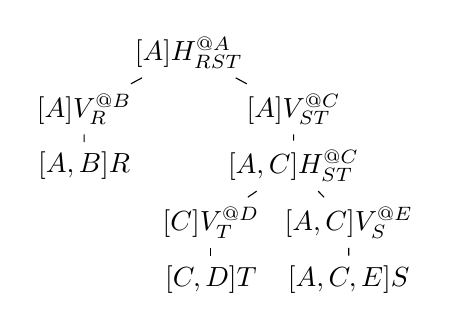
\begin{tikzpicture}[xscale=0.7, yscale=0.24]

    \node at (-0.4, 3) (A) {$\VIEW[A]{H^{@A}_{RST}}$};     
     \node at (1.5, 0) (C) {$\VIEW[A]{V^{@C}_{ST}}$} edge[-] (A);      
     \node at (1.5, -3) (C') {$\VIEW[A,C]{H^{@C}_{ST}}$} edge[-] (C);      
     \node at (2.5, -6) (E) {$\VIEW[A,C]{V^{@E}_{S}}$} edge[-] (C');
      \node at (2.5, -9) {$\VIEW[A,C,E]{S}$} edge[-] (E);
    
    \node at (0, -6) (D) {$\VIEW[C]{V^{@D}_{T}}$} edge[-] (C');
      \node at (0, -9) {$\VIEW[C,D]{T}$} edge[-] (D);  

      \node at (-2.3, -0) (B) {$\VIEW[A]{V^{@B}_{R}}$} edge[-] (A);
      \node at (-2.3, -3) {$\VIEW[A,B]{R}$} edge[-] (B);  
\end{tikzpicture}
% }
\hspace{0.5cm}
% \scalebox{0.87}{
  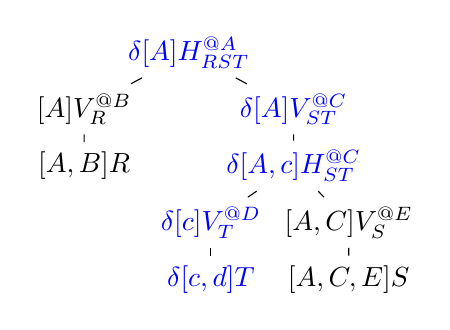
\begin{tikzpicture}[xscale=0.7, yscale=0.24]

    \node at (-0.4, 3) (A) {\color{blue} $\delta\VIEW[A]{H^{@A}_{RST}}$};     
     \node at (1.5, 0) (C) {\color{blue} $\delta\VIEW[A]{V^{@C}_{ST}}$} edge[-] (A);      
     \node at (1.5, -3) (C') {\color{blue} $\delta\VIEW[A,c]{H^{@C}_{ST}}$} edge[-] (C);      
     \node at (2.5, -6) (E) {$\VIEW[A, C]{V^{@E}_{S}}$} edge[-] (C');
      \node at (2.5, -9) {$\VIEW[A, C ,E]{S}$} edge[-] (E);
    
    \node at (0, -6) (D) {$\color{blue} \delta\VIEW[c]{V^{@D}_{T}}$} edge[-] (C');
      \node at (0, -9) {$\color{blue} \delta\VIEW[c,d]{T}$} edge[-] (D);  

      \node at (-2.3, -0) (B) {$\VIEW[A]{V^{@B}_{R}}$} edge[-] (A);
      \node at (-2.3, -3) {$\VIEW[A,B]{R}$} edge[-] (B);  
\end{tikzpicture}
% }
\caption{(left) View tree constructed by the function $\nu$ in 
Figure~\ref{fig:static_view_tree_algo_free-connex} for the variable 
order $\omega$ in Figure~\ref{fig:example_payloads};
(right) Delta view tree for a single-tuple update to $\VIEW{T}$.}
\label{fig:free-connex_view_tree}
% \vspace*{-1.45em}
\end{figure}

%\paragraph{\textbf{Updates}}
\textbf{Updates.} 
 The construction of delta view trees under single-tuple updates
 is exactly as described 
by the function $\Delta$ in Figure~\ref{fig:dynamic_view_tree_algo} (Section~\ref{sec:factorized_IVM}).
Since the view trees can be constructed in linear time, 
%and a single-tuple update to a relation fixes the variables of the relation schema
%in all ancestor views to constants, 
the delta view trees can also be constructed in linear time.

\begin{example}
Continuing Example~\ref{ex:free-connex-viewtree}, we consider a single-tuple update $\delta\VIEW{T}[c,d]$ to relation $\VIEW{T}$.
Figure~\ref{fig:free-connex_view_tree} depicts the original view tree (left) and the delta view tree for updates to $\VIEW{T}$ (right). The difference is that along the path from $\VIEW{T}$ to the root, we now have delta views.
The delta view $\delta\VIEW[]{V^{@D}_{T}}$
results from  $\delta\VIEW[c,d]{T}$ by marginalizing $D$, which takes  
constant time since $D$ is fixed to the constant $d$.
To compute $\delta\VIEW[]{H^{@C}_{ST}}$, we iterate over all $A$-values 
paired with $c$ in $\VIEW[]{V^{@E}_{S}}$. This operation takes linear time with the support of an index on variable $C$ built for this view.
% can be done in linear time with support of a tertiary index on variable $C$ for this view.
We obtain $\delta\VIEW[]{V^{@C}_{ST}}$ from $\delta\VIEW[]{H^{@C}_{ST}}$
by marginalizing the variable $C$. This requires constant time because $C$ is fixed to
the constant $c$. 
The top delta view $\delta\VIEW[]{H^{@A}_{RST}}$ is obtained by intersecting the two child views, e.g., by iterating over $\delta\VIEW[]{V^{@C}_{ST}}$ and doing lookups in $\VIEW[]{V^{@B}_R}$. This requires linear time. We conclude that the delta views can be computed in linear time. 
\punto
\end{example}

%\paragraph{\textbf{Enumeration.}}
\textbf{Enumeration.} 
Consider a view tree $\tau$ constructed using the function $\nu$ from 
Figure~\ref{fig:static_view_tree_algo_free-connex} for a free-top variable order of a 
query $\VIEW[]{Q}$. 
We first describe how to enumerate with constant delay the distinct tuples in the result of $\VIEW{Q}$ using $\tau$. Then, we explain how to compute the payload of each result tuple in constant time. 


Let $X_1, \ldots, X_n$ be an ordering of the free variables of the query
that is compatible with a top-down traversal of the free-top variable order. 
We use the views $\VIEW[]{V_1}, \ldots , \VIEW[]{V_n}$
%$\VIEW[]{H^{@X_1}}, \ldots , \VIEW[]{H^{@X_n}}$ 
to enumerate the distinct tuples
in the result of $\VIEW[]{Q}$, where 
$\VIEW[]{V_j}$ is $\VIEW[]{H^{@X_j}_{rels}}$ if $X_j$ has at least two children
and it is the child view of $X_j$ otherwise.  
We retrieve from $\VIEW[]{V_1}$ the first $X_1$-value in the 
result. 
When we arrive at a view  $\VIEW[]{V_j}$ with $j > 1$, we have already fixed 
the values of the variables above $X_j$ in the variable order. 
We retrieve from $\VIEW[]{V_j}$ the first $X_j$-value paired with these values. 
Once the values over all free variables 
are fixed, we have a complete result tuple that we output.
Then, we iterate over the remaining distinct $X_n$-values in $\VIEW[]{V_n}$
paired with the fixed values over the ancestor variables of $X_n$
and output a new tuple for each such value.
After all $X_n$-values are exhausted, we backtrack, i.e., we move to the next $X_{n-1}$-value
and restart the iteration of the matching $X_n$-values.      



\begin{figure}[t]
\centering
\setlength{\tabcolsep}{3pt}
%
\begin{tabular}{@{}c@{}c@{~~~}l}
  \toprule
  \multicolumn{3}{c}{$payload$(\text{view tree} $\tau$, \text{tuple} \textvec{t}): \text{payload}} \\
  \midrule
  \multicolumn{3}{l}{\MATCH $\tau$:} \\
  \midrule 
  \phantom{a} & $\VIEW{R}$\hspace*{2.5em} & \RETURN $\VIEW{R}(\textvec{t})$ \\
  \cmidrule{2-3} \\[-6pt] 
  &
  \begin{minipage}[b]{1.5cm}
    \begin{tikzpicture}[xscale=0.4, yscale=1]
      \node at (0,-2)  (n4) {$\VIEW[\mathcal{X}]{V}$};
      \node at (-1,-3)  (n1) {$\tau_1$} edge[-] (n4);
      \node at (0,-3)  (n2) {$\ldots$};
      \node at (1,-3)  (n3) {$\tau_k$} edge[-] (n4);
      \node at (0,-4.5) {~};
    \end{tikzpicture}
    \vspace{-0.9cm} 
  \end{minipage}
  &
\begin{minipage}[b]{6.2cm} 
\IF $\mathcal{X} = \sch(\textvec{t})$\\[0.5ex]
\TAB \RETURN $\VIEW{V}(\textvec{t})$\\[0.5ex]
\ELSE \ // $\mathcal{X} \subset \sch(\textvec{t})$ \\[0.5ex]
   \TAB \LET $\mathcal{V}_i =$ variables in $\tau_i$, \ $\forall i \in [k]$ \\[0.5ex]
    \TAB \RETURN $\prod_{i \in [k]} payload(\tau_i, \pi_{\mathcal{V}_i}\textvec{t})$
  \end{minipage}
  \\
  \bottomrule
\end{tabular}
\caption{Computing the payload of a tuple from a view tree.}
\label{fig:payload_computation}
\end{figure}

Given a complete tuple $\textvec{t}$ constructed from the view tree $\tau$, we use the 
function $payload$ from Figure~\ref{fig:payload_computation} to compute its payload. 
The function first checks whether the schema of the root view is exactly the schema 
$\sch(\textvec{t})$ of $\textvec{t}$. If so, it returns the payload of $\textvec{t}$ in this view. Otherwise, the root view covers only a subset of the schema of the tuple. 
In this case, the function recursively computes the payload for each subtree $\tau_i$ of the root view
and the projection of $\textvec{t}$ onto the variables in $\tau_i$.
The final payload is the product of the payloads returned for the subtrees. 
The returned payloads are from the lowest views in the view tree whose schemas consist of free variables only. If all variables are free, then these lowest views are the input relations themselves. 


\begin{remark}
The enumeration procedure needs the payloads of the lowest views whose schemas consist of free variables. The payloads from the views above these views thus need not be maintained, beyond keeping track of the multiplicities of each of their tuples. The maintenance of multiplicities is important for correctness, as it tells whether a tuple is to be removed from a view or still has at least one possible derivation from the input. 
For expensive payloads, such as those introduced in Section~\ref{sec:applications}, it is therefore more efficient to only maintain them for the views from the input relations up to the views used to compute the payloads. Their ancestor views only need maintenance of tuple multiplicities.\punto
\end{remark}

\begin{example}
We enumerate the distinct result tuples of the query
$\VIEW[A,B,C]{Q}$ 
from Example~\ref{ex:acyclic} using the view tree in Figure~\ref{fig:free-connex_view_tree} (left). We iterate with constant delay 
over the $A$-values in $\VIEW[A]{H^{@A}_{RST}}$. For each such $A$-value
$a$, we iterate with constant delay over the $B$-values in 
$\VIEW[a,B]{R}$ and over the $C$-values in 
$\VIEW[a,C]{H^{@C}_{ST}}$. Each triple $(a,b,c)$
obtained in this way is a result tuple of $\VIEW[]{Q}$.
Its payload is $\VIEW[a,b]{R} \cdot \VIEW[a,c]{H^{@C}_{ST}}$.  
\punto
\end{example}
\begin{remark}
  To efficiently support enumeration and updates, we may need several indices for the views in a view tree for a free-connex acyclic query. Each view  (and input relation) in the view tree in Figure~\ref{fig:free-connex_view_tree} (left) needs an index that can retrieve the payload for a given tuple of values over its variables. This is a primary index. For (top-down) enumeration, we may also need a secondary index per view to lookup for tuples that have as prefix a tuple of values over the variables shared with its parent view. Yet in case of some views, we may also need a tertiary index to support updates, which are propagated bottom-up. 
  %
  For instance, the view $\VIEW[A,C]{V^{@E}_{S}}$ requires: a primary index to retrieve the payload for each $(A,C)$-tuple; a secondary index to enumerate the $C$-values paired with a given $A$-value fixed by the parent view; and a tertiary index to obtain all $A$-values paired with a given $C$-value $c$ fixed by the delta of its left sibling $\delta\VIEW[c]{V^{@D}_{T}}$. All other views only require primary and secondary indices and no tertiary index.\punto
\end{remark}



\subsection{$Q$-Hierarchical Queries}
\label{sec:q-hierarchical}

$Q$-hierarchical queries form a strict subclass of the free-co\-nnex acyc\-lic queries.
They admit linear preprocessing time, constant update time, and constant enumeration delay~\cite{Nicole:PODS:2017}. Under widely-held complexity theoretic assumptions, there is no algorithm that achieves constant update time and enumeration delay for queries that are not $q$-hierarchical and have no repeating relation symbols~\cite{Nicole:PODS:2017}.
\DF recovers the aforementioned complexities using exactly the same approach as for free-connex acyclic queries detailed in Section~\ref{sec:free-connex}. This directly implies linear preprocessing time and  constant enumeration delay. Constant update time follows from the following observation. Every $q$-hierarchical query admits a free-top variables order, where each root-to-leaf path consists of variables that represent precisely the schema of a relation in the query. A single-tuple update to that relation then sets all these variables to constants, effectively making each delta view along that path of constant size. Our view tree construction also ensures that the computation of each delta view only requires one constant-time lookup per child view.

We first define $q$-hierarchical queries and then show how \DF achieves constant-time update for them. 
For a variable $X$ in a query, we denote by $\textsf{rels}(X)$ the set of relations that contain $X$ in their schema.
\begin{definition}[\cite{Suciu:PDB:11,Nicole:PODS:2017}]
   A query is \emph{hierarchical} if for any two variables $X$ and $Y$, it holds $\textsf{rels}(X) \subseteq \textsf{rels}(Y)$, $\textsf{rels}(Y) \subseteq \textsf{rels}(X)$, or $\textsf{rels}(X) \cap \textsf{rels}(Y) = \emptyset$. 

   A query is \emph{$q$-hierarchical} if it is hierarchical and for any  two variables $X$ and $Y$,
   it holds: if $\textsf{rels}(X) \supset \textsf{rels}(Y)$ and $Y$ is free, then $X$ is free.
\end{definition}

 Every $q$-hierarchical query admits a {\em canonical free-top} variable order, where (i) each root-to-leaf path consists of variables that form the schema of a relation and (2) no bound variable is above a free variable~\cite{KNOZ20}.
We can construct such a variable order in polynomial time in the query size as follows.
We start with the empty variable order.
For each relation $R$, we add to the variable order a root-to-leaf path made up of $R$'s variables ordered  as follows:  
a variable $X$ is before a variable $Y$ if (1) $\textsf{rels}(X) \supset \textsf{rels}(Y)$
or (2) $\textsf{rels}(X) \not\supset \textsf{rels}(Y)$, $\textsf{rels}(X) \not\subset \textsf{rels}(Y)$, $X$ is free, and $Y$ is bound. 

 \begin{figure}[t]
    % \hspace{0.2cm}%\centering
    \centering
    \begin{minipage}[b]{0.3\linewidth}
    % \scalebox{0.9}{
      \begin{tikzpicture}[xscale=0.96, yscale=0.8]
        \node at (0, 0.0) (A) {\small  $A$};
        \node at (-0.4, -1.0) (B) {\small $B$}  edge[-] (A);
        \node at (0.4, -1.0) (C) {\small $C$} edge[-] (A);
        \node at (0.8, -2.0) (E) {\small $E$} edge[-] (C);
        \node at (0, -2.0) (D) {\small $D$} edge[-] (C);
        \node at (0.8, -2.6) (S) {\small $S$};
        \node at (-0.6, -1.55) (R) {\small  $R$};
        \node at (-0.1, -2.6) (T) {\small  $T$};
                \node at (2.3, -1.5) {\scalebox{0.9} {
        \begin{tabular}{@{~~~~}l}
          $dep(A) = \emptyset$\\[1ex]
          $dep(B)=\{A\}$\\[1ex]
          $dep(C)=\{A\}$\\[1ex]
          $dep(D)=\{A,C\}$\\[1ex]
          $dep(E)=\{A,C\}$\\[8ex]
        \end{tabular}
      }};
        \begin{pgfonlayer}{background}
          \draw[opacity=.5,fill opacity=.5,line cap=round, line join=round, line width=15pt,color=teal] (0,0.0) -- (-0.4,-1);
          \draw[opacity=.5,fill opacity=.5,line cap=round, line join=round, line width=18pt,color=orange] (0,0.0) -- (0.8,-2.0);
          \draw[opacity=.5,fill opacity=.5,line cap=round, line join=round, line width=15pt,color=yellow] (0,0.0) -- (0.4,-1) -- (0, -2.0);
        \end{pgfonlayer}
      \end{tikzpicture}
      % }
    \end{minipage}
  \hspace{1.2cm}
    \begin{minipage}[b]{0.4\linewidth}
    % \scalebox{0.9}{
  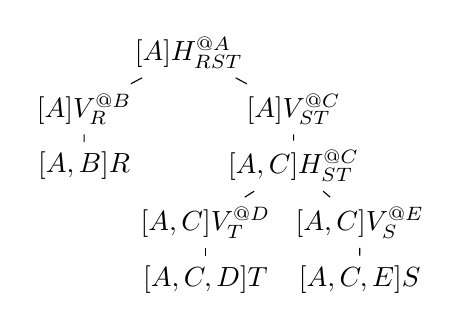
\begin{tikzpicture}[xscale=0.7, yscale=0.24]

    \node at (-0.4, 3) (A) {$\VIEW[A]{H^{@A}_{RST}}$};     
     \node at (1.5, 0) (C) {$\VIEW[A]{V^{@C}_{ST}}$} edge[-] (A);      
     \node at (1.5, -3) (C') {$\VIEW[A,C]{H^{@C}_{ST}}$} edge[-] (C);      
     \node at (2.7, -6) (E) {$\VIEW[A,C]{V^{@E}_{S}}$} edge[-] (C');
      \node at (2.7, -9) {$\VIEW[A,C,E]{S}$} edge[-] (E);
    
    \node at (-0.1, -6) (D) {$\VIEW[A,C]{V^{@D}_{T}}$} edge[-] (C');
      \node at (-0.1, -9) {$\VIEW[A,C,D]{T}$} edge[-] (D);  

      \node at (-2.3, -0) (B) {$\VIEW[A]{V^{@B}_{R}}$} edge[-] (A);
      \node at (-2.3, -3) {$\VIEW[A,B]{R}$} edge[-] (B);  
    \end{tikzpicture}
% }
    \end{minipage}
    \caption{(left) Canonical free-top variable order of the query $\VIEW[]{Q_h}$ from Example 
    \ref{ex:hierarchical}; 
    (right) Corresponding view tree.}
    \label{fig:q-hierarchical_view_tree}
    \end{figure}
    
\begin{example}
\label{ex:hierarchical}
The free-connex acyclic query 
$\VIEW[A,B,C]{Q}$ $=$ 
$\VSUM_{D}\VSUM_{E}$ $\VIEW[A,B]{R} \VPROD \VIEW[A,C,E]{S} \VPROD \VIEW[C,D]{T}$
from Example~\ref{ex:acyclic} is not hierarchical: the sets $\textsf{rels}(A)= \{\VIEW[]{R} , \VIEW[]{S}\}$
$\textsf{rels}(C)= \{\VIEW[]{S} , \VIEW[]{T}\}$ are not disjoint, nor one is included in the other.
By extending the schema of $\VIEW[]{T}$ with $A$, we obtain the $q$-hierarchical query 
$\VIEW[A,B,C]{Q_h}$ $=$ 
$\VSUM_{D}\VSUM_{E}$ $\VIEW[A,B]{R} \VPROD \VIEW[A,C,E]{S} \VPROD \VIEW[A,C,D]{T}$
whose canonical free-top variable order is given in Figure~\ref{fig:q-hierarchical_view_tree} (left).
The variant of the query,  
where variable $A$ is bound is hierarchical but not $q$-hierarchical because  
the set $\mathsf{rels}(A)= \{\VIEW[]{R}, \VIEW[]{S}, \VIEW[]{T}\}$ 
for the  \emph{bound} variable  $A$ is a strict superset of the set 
$\mathsf{rels}(B)= \{\VIEW[]{R}\}$ for the \emph{free} variable $B$.
\punto
\end{example}
     
We next exemplify  how \DF achieves constant-time update for a $q$-hierarchical query.       
   
\begin{example}\label{ex:qhierarchical-update}
Figure~\ref{fig:q-hierarchical_view_tree} shows the view tree (right)
modeled on the canonical free-top variable order (left) of the 
$q$-hierarchical query $\VIEW[]{Q_h}$ in Example~\ref{ex:hierarchical}.
Figure~\ref{fig:q-hierarchical_delta_view_trees} shows the
delta view trees under single-tuple updates to $\VIEW[]{R}$  and $\VIEW[]{T}$.

In the delta view tree for $\VIEW[]{R}$, the delta view
$\delta \VIEW[]{H^{@A}_{RST}}$ can be computed by  a constant-time lookup in 
$\VIEW[]{V^{@C}_{ST}}$.   
In the delta view tree for $\VIEW[]{T}$, the delta views
$\delta \VIEW[]{H^{@C}_{ST}}$ and $\delta \VIEW[]{H^{@A}_{RST}}$ 
can be computed by constant-time lookups in 
$\VIEW[]{V^{@E}_{S}}$ and $\VIEW[]{V^{@B}_{R}}$, respectively. 
All other delta views are computed by marginalizing a variable with a single value. 
\punto
\end{example}

\begin{figure}[t]
    \hspace{-0.15cm}
    \centering
    \begin{minipage}[b]{0.3\linewidth}
    % \scalebox{0.87}{
  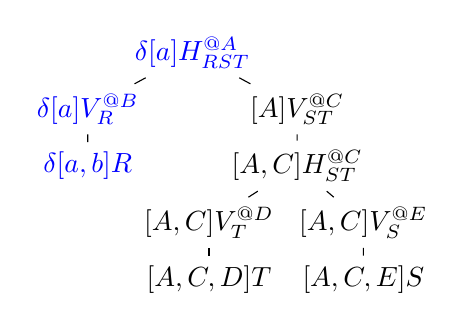
\begin{tikzpicture}[xscale=0.7, yscale=0.24]

    \node at (-0.4, 3) (A) {$\color{blue} \delta \VIEW[a]{H^{@A}_{RST}}$};     
     \node at (1.5, 0) (C) {$\VIEW[A]{V^{@C}_{ST}}$} edge[-] (A);      
     \node at (1.5, -3) (C') {$\VIEW[A,C]{H^{@C}_{ST}}$} edge[-] (C);      
     \node at (2.7, -6) (E) {$\VIEW[A,C]{V^{@E}_{S}}$} edge[-] (C');
      \node at (2.7, -9) {$\VIEW[A,C,E]{S}$} edge[-] (E);
    
    \node at (-0.1, -6) (D) {$\VIEW[A,C]{V^{@D}_{T}}$} edge[-] (C');
    \node at (-0.1, -9) {$\VIEW[A,C,D]{T}$} edge[-] (D);  

      \node at (-2.3, -0) (B) {$\color{blue}\delta \VIEW[a]{V^{@B}_{R}}$} edge[-] (A);
      \node at (-2.3, -3) {$\color{blue}\delta \VIEW[a,b]{R}$} edge[-] (B);  
\end{tikzpicture}
% }
    \end{minipage}
  \hspace{1.5cm}
    \begin{minipage}[b]{0.4\linewidth}
    % \scalebox{0.87}{
  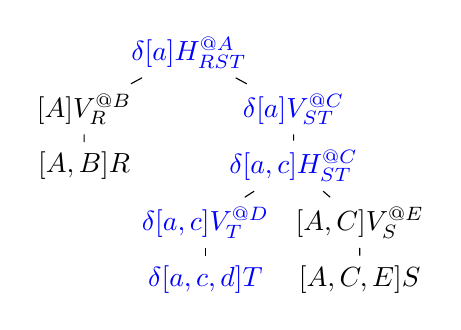
\begin{tikzpicture}[xscale=0.7, yscale=0.24]

    \node at (-0.4, 3) (A) {$\color{blue} \delta \VIEW[a]{H^{@A}_{RST}}$};     
     \node at (1.5, 0) (C) {$\color{blue}\delta \VIEW[a]{V^{@C}_{ST}}$} edge[-] (A);      
     \node at (1.5, -3) (C') {\color{blue}$\delta \VIEW[a,c]{H^{@C}_{ST}}$} edge[-] (C);      
     \node at (2.7, -6) (E) {$\VIEW[A,C]{V^{@E}_{S}}$} edge[-] (C');
      \node at (2.7, -9) {$\VIEW[A,C,E]{S}$} edge[-] (E);
    
    \node at (-0.1, -6) (D) {$\color{blue}\delta \VIEW[a,c]{V^{@D}_{T}}$} edge[-] (C');
    \node at (-0.1, -9) {$\color{blue}\delta \VIEW[a,c,d]{T}$} edge[-] (D);  

    \node at (-2.3, -0) (B) {$\VIEW[A]{V^{@B}_{R}}$} edge[-] (A);
    \node at (-2.3, -3) {$\VIEW[A,B]{R}$} edge[-] (B);  
\end{tikzpicture}
% }
    \end{minipage}
    \caption{Delta view trees derived from the view tree in Figure~\ref{fig:q-hierarchical_view_tree} 
for single-tuple updates to relations $\VIEW[]{R}$ (left) and $\VIEW[]{T}$ (right).}
    \label{fig:q-hierarchical_delta_view_trees}
    \end{figure}
 
\begin{remark}
  $Q$-hierarchical queries admit view trees who\-se views only need primary indices to support payload lookup and updates and possibly secondary indices to support enumeration.
  Consider the view tree in Figure~\ref{fig:q-hierarchical_view_tree}. Enumeration proceeds top-down: We iterate over the $A$-values in the top view and for each such value $a$, 
  %we look up in $\VIEW[a]{V^{@B}_{R}}$ and $\VIEW[a]{V^{@C}_{ST}}$, then continue to 
  we look up in $\VIEW[a,B]{R}$ to enumerate over all the $B$-values paired with $a$, and also look up into $\VIEW[a,C]{H^{@C}_{ST}}$ to enumerate over all $C$-values paired with $a$. %We continue similarly to get all $D$-values and $E$-values paired with $a$ and each $C$-value. 
  All these look-ups require primary or secondary indices.  
  
  
  Figure~\ref{fig:q-hierarchical_delta_view_trees} shows the delta view trees for single-tuple updates to $\VIEW[]{R}$ and $\VIEW[]{T}$. To compute a delta view along the path from the delta relation to the root of the delta view tree, we either perform a projection on a delta view or a lookup in the primary index of a sibling view (so with all keys of the index set to constants).\punto
\end{remark}

%%%%%%%%%%%%%%%%%%%%%%%%%%%%%%%%%
\subsection{Queries under Functional Dependencies}

Non-hierar\-chical queries may become hierarchical under functional dependencies (fds)~\cite{OlteanuHK09}.

Given a set $\Sigma$ of fds, we denote by $\textsf{CLOSURE}_\Sigma(\calS)$ the closure of the set $\calS$ of variables under $\Sigma$~\cite{AbiteboulHV95}. For instance, given the fds $\Sigma=\{A\rightarrow D;BD \rightarrow E\}$, we have $\textsf{CLOSURE}_\Sigma(\{A,B,C\})=\{A,B,C,D,E\}$.

\begin{definition}[adapted from~\cite{OlteanuHK09}]
  Given a set $\Sigma$ of fds and a query $\VIEW[\calS]{Q} = \VSUM_{\calB} \VIEW[\calS_1]{R_1}\VPROD\cdots\VPROD\VIEW[\calS_n]{R_n}$, the \emph{$\Sigma$-reduct} of $\VIEW[]{Q}$ under $\Sigma$ is:
\begin{align*}
  \;
  \VIEW[\textsf{CLOSURE}_\Sigma(\calS)]{Q} = \VSUM_{\calB} &\VIEW[\textsf{CLOSURE}_\Sigma(\calS_1)]{R_1}\VPROD\cdots\VPROD \VIEW[\textsf{CLOSURE}_\Sigma(\calS_n)]{R_n}
\end{align*}
\end{definition}
The $\Sigma$-reduct of a query is thus another query, where the schema of each relation is extended to include all variables in the closure of this schema under $\Sigma$. Since the added variables are functionally determined by the original schema, they do not add more information. So, we could extend these schemas and the underlying database without increasing the number of tuples in the relations. For any database $D$ with fds $\Sigma$ and a query $\VIEW[]{Q}$, the query result $\VIEW[]{Q}(D)$ is the same as the result of its $\Sigma$-reduct over the extended database.
The benefit of this rewriting is that queries may admit free-connex acyclic or even $q$-hierarchical $\Sigma$-reducts. We need not physically extend the database to reap this benefit. Instead, we use the $\Sigma$-reduct of $\VIEW[]{Q}$ to infer a free-top variable order or even a canonical free-top variable order \emph{for} $\VIEW[]{Q}$ in case the $\Sigma$-reduct is free-connex acyclic or $q$-hierarchical, respectively.
Using this variable order, we construct a view tree for $\VIEW[]{Q}$ that enjoys the preprocessing, update, and enumerate times as for its $\Sigma$-reduct.

Theorem~\ref{th:special-cases} can be generalized to account for fds.

\begin{theorem}\label{th:special-cases-fds}
  Let a query $\VIEW[]{Q}$ and a database of size $N$ and with a set $\Sigma$ of functional dependencies.

  \DF can maintain $\VIEW[]{Q}$ with $O(N)$ preprocessing, $O(1)$ enumeration delay, and $O(N)$ single-tuple updates in case the $\Sigma$-reduct of $\VIEW[]{Q}$ is free-connex acyclic.
    
  \DF can maintain $\VIEW[]{Q}$ with $O(N)$ preprocessing, $O(1)$ enumeration delay, and $O(1)$ single-tuple updates in case the $\Sigma$-reduct of $\VIEW[]{Q}$ is $q$-hierarchical.
\end{theorem}

  \begin{figure}[t]
   \hspace{-0.1cm}
   \centering
    \begin{minipage}[b]{0.2\linewidth}
    % \scalebox{0.88}{
      \begin{tikzpicture}[xscale=0.96, yscale=0.8]
        \node at (0, 0) (D) {\small  $D$};
        \node at (0, -1) (C) {\small $C$};
        \node at (0, -2) (B) {\small $B$};
        \node at (0, -3) (A) {\small $A$};
        
    \node at (-0.5, -0.5) (T) {\small  $\VIEW{T}$};    
        \node at (-0.5, -1.5) (S) {\small  $\VIEW{S}$};    
            \node at (-0.5, -2.5) (R) {\small  $\VIEW{R}$};    
\begin{pgfonlayer}{background}
\draw[opacity=.5,fill opacity=.5,line cap=round, line join=round, line width=13pt,color=purple] (0,0) -- (0,-1);\draw[opacity=0.7,fill opacity=0.7,line cap=round, line join=round, line width=13pt,color=orange] (0,-1) -- (0,-2.0);
\draw[opacity=.5,fill opacity=.5,line cap=round, line join=round, line width=13pt,color=teal] (0,-2) -- (0,-3);
        \end{pgfonlayer}
      \end{tikzpicture}
      % }
    \end{minipage}
  \hspace{-0.5cm}
\begin{minipage}[b]{0.2\linewidth}
    % \scalebox{0.88}{
      \begin{tikzpicture}[xscale=0.96, yscale=0.8]
        \node at (0, 0) (D) {\small  $D$};
        \node at (0, -1) (C) {\small $C$};
        \node at (0, -2) (B) {\small $B$};
        \node at (0, -3) (A) {\small $A$};
        
            \node at (-0.6, -0.5) (T) {\small  $\VIEW{T}$};    
        \node at (-0.6, -1.6) (S) {\small  $\VIEW{S}$};    
            \node at (-0.6, -2.9) (R) {\small  $\VIEW{R}$};    
\begin{pgfonlayer}{background}
\draw[opacity=.5,fill opacity=1,line cap=round, line join=round, line width=23pt,color=teal] (0,0) -- (0,-3);
\draw[opacity=1,fill opacity=1,line cap=round, line join=round, line width=18pt,color=orange] (0,0) -- (0,-2);
\draw[opacity=0.8,fill opacity=0.8,line cap=round, line join=round, line width=13pt,color=purple] (0,0) -- (0,-1);
        \end{pgfonlayer}
      \end{tikzpicture}
      % }
    \end{minipage}    
    \hspace{-0.2cm}
    \begin{minipage}[b]{0.3\linewidth}
    % \scalebox{0.88}{
      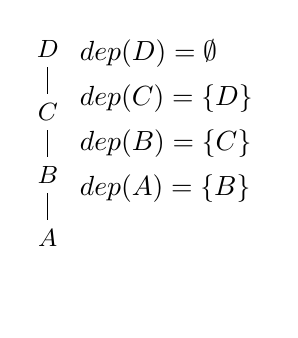
\begin{tikzpicture}[xscale=0.96, yscale=0.8]
        \node at (0, 0) (D) {\small  $D$};
        \node at (0, -1) (C) {\small $C$}edge[-] (D);
        \node at (0, -2) (B) {\small $B$}edge[-] (C);
        \node at (0, -3) (A) {\small $A$}edge[-] (B);
                   \node at (1.5, -1.9) {
        \begin{tabular}{@{~~}l}
          $dep(D)=\emptyset$\\[1ex]
          $dep(C)=\{D\}$\\[1ex]
          $dep(B)=\{C\}$\\[1ex]
          $dep(A)=\{B\}$\\[8ex]
        \end{tabular}
      }; 
      \end{tikzpicture}
      % }
      % \vspace{-0.2cm}
    \end{minipage}
    \hspace{0cm}
    \begin{minipage}[b]{0.2\linewidth}
    \scalebox{0.88}{
  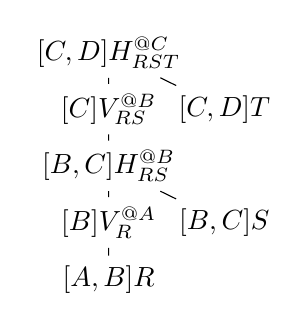
\begin{tikzpicture}[xscale=0.7, yscale=0.24]    
      \node at (-2.3, 6) (C) {$\VIEW[C,D]{H^{@C}_{RST}}$};
      \node at (-2.3, 3) (B) {$\VIEW[C]{V^{@B}_{RS}}$}edge[-] (C);
      \node at (-2.3, 0) (B') {$\VIEW[B,C]{H^{@B}_{RS}}$} edge[-] (B);
      \node at (-2.3, -3) (A) {$\VIEW[B]{V^{@A}_{R}}$}edge[-] (B');
      \node at (-2.3, -6) {$\VIEW[A,B]{R}$} edge[-] (A);  
      
            \node at (-0.2, -3) (S) {$\VIEW[B,C]{S}$}edge[-] (B');
      \node at (-0.2, 3) (T) {$\VIEW[C,D]{T}$}edge[-] (C);
\end{tikzpicture}
}
    \end{minipage}
    \caption{From left to right: Hypergraph of the query 
    $\VIEW{Q}$ and its $\Sigma$-reduct for $\Sigma = \{B \rightarrow C, C \rightarrow D\}$
    from Example~\ref{ex:q_hierarchical_rewriting}; 
    canonical variable order $\omega$ for  $\VIEW{Q}$; view tree modeled on $\omega$.}
    \label{fig:q-hierarchical_rewriting} 
    \end{figure}

%%%%%%%%%%%%%%%
    
  \begin{figure}[t]
 \hspace{-0.2cm}
 \centering
    \begin{minipage}[b]{0.2\linewidth}
    % \scalebox{0.93}{
  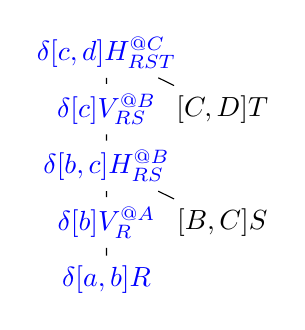
\begin{tikzpicture}[xscale=0.7, yscale=0.24]    
      \node at (-2.3, 6) (C) {\color{blue}$\delta\VIEW[c,d]{H^{@C}_{RST}}$};
      \node at (-2.3, 3) (B) {\color{blue}$\delta\VIEW[c]{V^{@B}_{RS}}$}edge[-] (C);
      \node at (-2.3, 0) (B') {$\color{blue}\delta\VIEW[b,c]{H^{@B}_{RS}}$} edge[-] (B);
      \node at (-2.3, -3) (A) {$\color{blue}\delta\VIEW[b]{V^{@A}_{R}}$}edge[-] (B');
      \node at (-2.3, -6) {$\color{blue}\delta\VIEW[a,b]{R}$} edge[-] (A);  
      
            \node at (-0.2, -3) (S) {$\VIEW[B,C]{S}$}edge[-] (B');
      \node at (-0.2, 3) (T) {$\VIEW[C,D]{T}$}edge[-] (C);
\end{tikzpicture}
% }
    \end{minipage}
    \hspace{1cm}
    \begin{minipage}[b]{0.2\linewidth}
    % \scalebox{0.93}{
  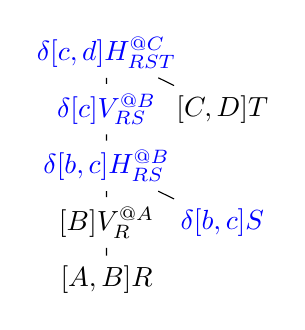
\begin{tikzpicture}[xscale=0.7, yscale=0.24]    
      \node at (-2.3, 6) (C) {\color{blue} $\delta\VIEW[c,d]{H^{@C}_{RST}}$};
      \node at (-2.3, 3) (B) {\color{blue}$\delta\VIEW[c]{V^{@B}_{RS}}$}edge[-] (C);
      \node at (-2.3, 0) (B') {\color{blue}$\delta\VIEW[b,c]{H^{@B}_{RS}}$} edge[-] (B);
      \node at (-2.3, -3) (A) {$\VIEW[B]{V^{@A}_{R}}$}edge[-] (B');
      \node at (-2.3, -6) {$\VIEW[A,B]{R}$} edge[-] (A);  
      
            \node at (-0.2, -3) (S) {\color{blue}$\delta\VIEW[b,c]{S}$}edge[-] (B');
      \node at (-0.2, 3) (T) {$\VIEW[C,D]{T}$}edge[-] (C);
\end{tikzpicture}
% }
    \end{minipage}
    \hspace{1cm}
    \begin{minipage}[b]{0.2\linewidth}
    % \scalebox{0.93}{
  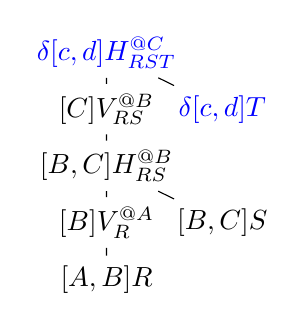
\begin{tikzpicture}[xscale=0.7, yscale=0.24]    
      \node at (-2.3, 6) (C) {\color{blue}$\delta\VIEW[c,d]{H^{@C}_{RST}}$};
      \node at (-2.3, 3) (B) {$\VIEW[C]{V^{@B}_{RS}}$}edge[-] (C);
      \node at (-2.3, 0) (B') {$\VIEW[B,C]{H^{@B}_{RS}}$} edge[-] (B);
      \node at (-2.3, -3) (A) {$\VIEW[B]{V^{@A}_{R}}$}edge[-] (B');
      \node at (-2.3, -6) {$\VIEW[A,B]{R}$} edge[-] (A);  
      
            \node at (-0.2, -3) (S) {$\VIEW[B,C]{S}$}edge[-] (B');
      \node at (-0.2, 3) (T) {\color{blue}$\delta\VIEW[c,d]{T}$}edge[-] (C);
\end{tikzpicture}
% }
    \end{minipage}
    \caption{Delta view trees derived from the view tree in Figure~\ref{fig:q-hierarchical_rewriting} for single-tuple updates to 
% $\VIEW{R}$ (left), $\VIEW{S}$ (middle), and $\VIEW{T}$ (right). 
$\VIEW{R}$, $\VIEW{S}$, and $\VIEW{T}$ (left to right). 
The values $b$ and $c$ functionally determine $c$ and $d$, respectively.}
    \label{fig:q-hierarchical_rewriting_delta}
    \end{figure}
    
\begin{example} 
\label{ex:q_hierarchical_rewriting}
Consider $\Sigma = \{B \rightarrow C, C \rightarrow D\}$ and the free-connex acyclic but not hierarchical query
\begin{align*}
\quad  \VIEW[A,B,C,D]{Q} =\VIEW[A,B]{R} \VPROD \VIEW[B,C]{S} \VPROD \VIEW[C,D]{T}.
\end{align*}
The $\Sigma$-reduct of $\VIEW[]{Q}$ is 
\begin{align*}
\VIEW[A,B,C,D]{Q'} \hspace{-0.1em} =\VIEW[A,B,C,D]{R} \VPROD \VIEW[B,C,D]{S} \VPROD \VIEW[C,D]{T}.
\end{align*}
Figure~\ref{fig:q-hierarchical_rewriting} depicts the hypergraphs
of $\VIEW[]{Q}$ and $\VIEW[]{Q'}$ (left), a free-top variable order for 
$\VIEW[]{Q}$ that is also canonical for $\VIEW[]{Q'}$ (middle), and 
the view tree for $\VIEW[]{Q}$ modeled on this variable order (right).
Since $\VIEW{Q}$ is free-connex acylic, we can compute the view tree in linear time and enumerate the result tuples of $\VIEW{Q}$ with constant delay, as explained in Section~\ref{sec:free-connex}. 
We next describe how to achieve constant-time update by exploiting 
  the fds. Figure~\ref{fig:q-hierarchical_rewriting_delta} shows the delta view trees obtained from the view tree for $\VIEW{Q}$ for single-tuple updates to $\VIEW{R}$, $\VIEW{S}$, and $\VIEW{T}$.

Consider first the update $\delta\VIEW[a,b]{R}$ to relation $\VIEW[]{R}$. The delta view $\delta\VIEW[b]{V^{@A}_{R}}$ is just a projection of the update tuple. The delta view $\delta\VIEW[b,c]{H^{@B}_{RS}}$ requires a lookup in $\VIEW[B,C]{S}$ for $B=b$. In general, there may be many $C$-values paired with $b$. However, under the fd $B\rightarrow C$, there is at most one $C$-value $c$ paired with $b$. Hence, the construction of this delta view takes constant time. Similarly, the delta view $\delta\VIEW[c,d]{H^{@C}_{RST}}$ requires a lookup in $\VIEW[C,D]{T}$ for $C=c$. Again, there may be many $D$-values paired with $c$, yet under the fd $C\rightarrow D$, there is at most one $D$-value $d$ paired with $c$. Hence, the construction of this delta view takes constant time, too.

Similar reasoning applies to the update $\delta\VIEW[b,c]{S}$. To compute the delta view $\delta\VIEW[c,b]{H^{@B}_{RS}}$, we need a constant-time lookup in the view $\VIEW[B]{V^{@A}_R}$ with $B=b$. Computing $\delta\VIEW[c,d]{H^{@C}_{RST}}$ takes constant time due to the fd $C\rightarrow D$, as with updates to  $\VIEW{R}$. 
Processing the update $\delta\VIEW[c,d]{T}$ takes constant time without exploiting the fds: it only requires a lookup in the view $\VIEW[C]{V^{@B}_{RS}}$ with $C=c$. \punto
\end{example} 
%%%%%%%%%%%%%%%%%%%%%%%%%%%%%%%%%%%%